\documentclass[12pt]{caltech_thesis}
\usepackage[hyphens]{url}
\usepackage{lipsum}
\usepackage{graphicx}
\usepackage{todonotes}
\usepackage[utf8]{inputenc}
\usepackage[T1]{fontenc}
\usepackage{mathpazo}
\usepackage[numbers,sort&compress]{natbib}
\usepackage{csquotes}
\usepackage{bibunits}
\usepackage{enumitem}
\usepackage{amsmath}
\usepackage{longtable}
\usepackage{xcolor}
\usepackage{indentfirst} 
\usepackage{upgreek}
\definecolor{CaltechOrange}{HTML}{FF6C0C}
\usepackage[hidelinks=true,
            colorlinks=true, 
            linkcolor=black,
            urlcolor=CaltechOrange, 
            linkbordercolor=white,
            backref=false,
            pagebackref=false,
            hyperindex=false,
            breaklinks=true,
            bookmarks=false,
            bookmarksopen=false,
            ]{hyperref}
\usepackage[
            backend=biber,natbib,
            % IMPORTANT: load a style suitable for your discipline
            style=ieee
        ]{biblatex}


% added to conform with this issue: https://github.com/jgm/pandoc/issues/4384
% with this, figure width can be changed with {width: 70%}
\makeatletter
\def\maxwidth{\ifdim\Gin@nat@width>\linewidth\linewidth\else\Gin@nat@width\fi}
\def\maxheight{\ifdim\Gin@nat@height>\textheight\textheight\else\Gin@nat@height\fi}
\makeatother
% Scale images if necessary, so that they will not overflow the page
% margins by default, and it is still possible to overwrite the defaults
% using explicit options in \includegraphics[width, height, ...]{}
\setkeys{Gin}{width=\maxwidth,height=\maxheight,keepaspectratio}

\hypersetup{
  colorlinks = true,
  linkcolor = black
}

\makeatletter
\let\@mycite\@cite
\def\@cite#1#2{{\hypersetup{linkcolor=black!60!black}[{#1\if@tempswa , #2\fi}]}}
\makeatother
            
\addbibresource{references.bib}
\defaultbibliographystyle{plainnat}
\renewcommand{\bibsection}{\section*{\refname}}
\usepackage{memhfixc}
\linespread{1.5}


\begin{document}

\title{Towards Precise Quantum Measurements with Superconducting
Nanowire Single Photon Detectors}
\author{Andrew Sterling Mueller}
\degreeaward{Doctor of Philosophy in Applied Physics}                 
\university{California Institute of Technology}    
\address{Pasadena, California}                     
\unilogo{caltech.png}                                 
\copyyear{2023}  
\defenddate{XXX 2023}   



\rightsstatement{Some rights reserved. This thesis is distributed under
a Creative Commons Attribution License CC-BY 4.0. All software used in
the analysis and generation of figures is distributed under an MIT
license. and is available on a GitHub repository
\href{https://github.com/sansseriff/phd\textunderscore thesis}{https://github.com/sansseriff/phd_thesis}}

\maketitle[logo]

\begin{acknowledgements}   
    \input{frontmatter/acknowledgements.md}
\end{acknowledgements}

\begin{abstract}
  \input{frontmatter/abstract.md} 
\end{abstract}

\extrachapter{Published Content and Contributions}
\begin{publishedcontent}
\input{frontmatter/published.md}
\end{publishedcontent}

\tableofcontents
\listoffigures
\listoftables
\printnomenclature
\mainmatter

\hypertarget{low-dark-count-rate-detection}{%
\chapter{Low Dark Count Rate
Detection}\label{low-dark-count-rate-detection}}

~~~~~~~~~~~~~~~~~~~~~~~~~~~~~~~~~~~~~~~~~~~~~~~

\hypertarget{introduction}{%
\section{Introduction}\label{introduction}}

\[ \require{upgreek} \] Time-resolved photon detection with low dark
counts is a vital technology in fields such as quantum information
processing, classical communication, quantum communication, and laser
ranging. Increasingly, research in these fields employs superconducting
nanowire single photon detectors (SNSPDs), which have been demonstrated
with system detection efficiency (\(\eta\)) of more than 90\%
\autocite{Reddy2020}, timing jitter (\(\Delta t\)) as low as 2.6 ps
\autocite{Korzh2020} and intrinsic dark count rates (\(D\)) in the
milli- to micro-hertz range \autocite{Hochberg2019}. However, quantum
communication applications require detection systems with performance
optimized across all three metrics simultaneously. The dimensionless
figure of merit \(H\) specifies this application-specific performance as
\(H = \frac{\eta}{(\Delta t D)}\) \autocite{Hadfield2009}.

Here, we focus on lowering the Dark Count Rate (DCR) of a telecom-band
SNSPD system by filtering thermal photons, without sacrificing
efficiency or jitter. We demonstrate a free-space coupled SNSPD with
sub-0.1 Hz DCR, 14 ps timing jitter, and 72\% total system detection
efficiency (SDE) by using a differential single-pixel SNSPD
\autocite{Colangelo2021} to image a single-mode fiber through an
optimized free-space filter stack.

\%HARDWARE

\begin{figure}[htbp]
\centering\includegraphics[width=\linewidth]{Hardware and Filters Squashed 2.pdf}
\caption{\small a) System hardware. ASPH: aspheric lens, %(Edmund Optics \#47-729)
SP1 \& SP2: custom short-pass filters, BP: band-pass filter, %(Semrock NIR01-1550/3-25),
BK7: glass windows, SMF: Single-mode fiber, PEL: Peltier element, LC: Liquid cooling block. b) Transmission spectra for the three filters utilized. c) Absorption spectrum for the SNSPD efficiency-enhancing optical stack.}
\label{fig:setup}
\end{figure}

\%We compare performance with a fiber-coupled configuration using the
same detector.

The highest system detection efficiencies have been achieved using
self-aligned fiber coupling where dark counts can be reduced using
cryogenic fiber looping \autocite{Cohen2015} or spliced narrow-band
filters \autocite{Boaron2018secure}. But it is difficult to achieve
strong filtering without losses at the target wavelength. Low-loss,
high-rejection filters are typically available as free-space components,
so some of the highest reported H-values were achieved with cryogenic,
fiber to free-space to fiber coupling, but exhibit an SDE of only a few
percent \autocite{Shibata2015}. The filtering method presented here
takes advantage of commercially-available filters, achieves a high
free-space coupling efficiency using a cryogenic lens, and is compatible
with both fiber and free-space optical inputs.

In this work, a single mode fiber is imaged onto the detector using two
f = 18.75 mm lenses. One lens collimates light from an optical fiber
face outside the cryostat (Photon Spot), and the other focuses light
onto the detector inside \autocite{Bellei:16}. In the collimated region
between, the beam passes though a series of short-pass filters and one
band-pass filter mounted at 4 K (Fig. \ref{fig:setup}a). One of the
short-pass filters is angled to avoid ghosting effects. The 40 K
radiation shield and outer cryostat housing are fitted with
anti-reflection coated BK7 windows. The filters are spring loaded to
prevent cracking at low temperatures. To minimize effects of stray
light, the interior of the 4 K shield was painted with mid-IR absorbing
paint (Aeroglaze Z306) \autocite{Persky1999}, while gaps between filters
and the windows were covered with metal tape.

The system is based on 1-inch optics, although the f = 18.75 mm lenses
lead to a \(1/e^2\) intensity diameter of about 5 mm in the collimated
region. To reduce the larger-than-required numerical aperture of the
system, painted 8 mm apertures (Acktar Spectral Black) were added in the
collimated region. These are large enough to allow minor alignment
adjustments --- by translating the exterior collimating lens --- without
vignetting.

\begin{figure}[htbp]
\centering
\centering\includegraphics[width=\linewidth]{DataFigure_6.pdf}
\caption{ \small a) Simulated photon flux at various temperatures with and without the 1550 nm bandpass filter (BP). b) Normalized photon count rate (PCR) and jitter measurements c) DCR, and calculated figure of merit $H$ versus bias current for both fiber-coupled and free space coupled configurations.}
\label{fig:false-color}
\end{figure}

We use four custom cryogenic short-pass filters, with pass-bands below
\(1.6 \ \mathrm{\upmu m}\) and \(1.9 \ \mathrm{\upmu m}\) (Andover
Corp.), both with transmission at 1550 nm of 98.8 ± 0.3\%. They reject
wavelengths shorter than \(3 \ \mathrm{\upmu m}\) through reflective
optical coatings, and attenuate longer wavelengths through material
absorption in the 12.7 mm-thick N-BK7 glass substrate. While the
bandpass filter (FWHM = 7 nm) was found to blue-shift by about 2 nm at
cryogenic temperatures, the passband was wide enough such that
significant attenuation was not observed at the original target
wavelength of 1550 nm. This filter is also sufficiently wide to avoid
Fourier-limited broadening of ultra-short laser pulses.

The filtering of the optical stack was modeled by assuming a black-body
emitter at 298 K and a field of view defined by the 18.75 mm focal
length of the cryogenic lens and the 8 mm diameter of the apertures. The
resulting spectrum was multiplied by the transmission of the filters
(Fig. \ref{fig:setup}b) and detector optical stack (Fig.
\ref{fig:setup}c). The model showed that two each of the 1.6
\{\textmu\}m and 1.9 \{\textmu\}m short pass filters were necessary to
suppress mid-infrared light to where it was no longer the dominant
source of dark counts. With the inclusion of the four shortpass filters,
the dominant source of dark counts is the spectral region near 1550 nm
as shown in Fig. \ref{fig:false-color}a, which also illustrates the
effect of the bandpass filter. Also evident in Fig.
\ref{fig:false-color}a is the strong dependence of DCR on the
temperature of the final surface outside the cryostat emitting thermal
radiation. This motivated the exterior cooling apparatus shown at the
bottom of Fig. \ref{fig:setup}a. The bulkhead holding the fiber
connector is cooled to around -2\(^\circ\)C using a Peltier element and
liquid cooling block. This addition reduced the system DCR from 0.4 Hz
to below 0.1 Hz. While dark counts from multiple spatial modes are
present in this system --- modes that would not be present in a purely
fiber based approach --- the external cooling technique works to
minimize their effect.

This work used a low-jitter, differential SNSPD \cite{Colangelo2021},
with an active area of 22 \(\times\) 15 \{\textmu\}m, formed by a
meander of 100 nm-wide and 5-nm-thick niobium nitride (NbN) nanowires on
a 500 nm pitch. A more conventional single-ended readout SNSPD of
similar area would also achieve low DCR in this coupling system, but
would likely achieve a lower performance metric \(H\) from
correspondingly higher jitter. The nanowire is embedded in an
efficiency-enhancing optical stack made of alternating layers of
TiO\(_2\) and SiO\(_2\) and a gold mirror layer. As shown in Fig.
\ref{fig:false-color}b and c, when fiber coupled (without any
fiber-based filtering methods applied), this detector achieved a
saturated SDE of \(84\% \pm 4.4 \%\) and a DCR of 20 Hz at a bias
current of 16 \{\textmu\}A.

~~~~~ As also shown in Fig. \ref{fig:false-color}b, the free-space
coupling system achieves up to \(72 \% \pm 3.7 \%\) SDE as measured from
the fiber outside the cryostat. The reduction in efficiency is likely
due to surface reflections in the free-space optics, and potential
misalignment in the optical baffles. The minimum DCR (Fig.
\ref{fig:false-color}c) at \(72 \%\) SDE is about 0.1 Hz, with a bias
current of 16 \(\mathrm{\upmu A}\). These metrics, with the jitter
measurements shown in Fig. \ref{fig:false-color}b, give a maximum H
value of \(5 \times 10^{11}\) (Fig. \ref{fig:false-color}c). Values as
high as \(1.8 \times 10^{12}\) have been reported before, but at 1.5\%
system detection efficiency \cite{Shibata2015}. Our system shows a low
DCR can be achieved without severe reduction of SDE or usable target
wavelength bandwidth. This is paramount for the future of terrestrial
and space-to-ground quantum communication, since it increases success
rate with finite statistics \cite{Boaron2018secure}. The same techniques
can be applied to emerging SNSPD applications at longer wavelengths,
such as laser ranging \cite{Taylor2019}, where fiber filtering is
impractical. Beyond single-mode applications, our work paves the way to
scalable, low-DCR, multi-mode coupling to SNSPD arrays
\cite{Wollman2019}.

\hypertarget{fig:custom_figure}{%
\begin{figure}
\centering
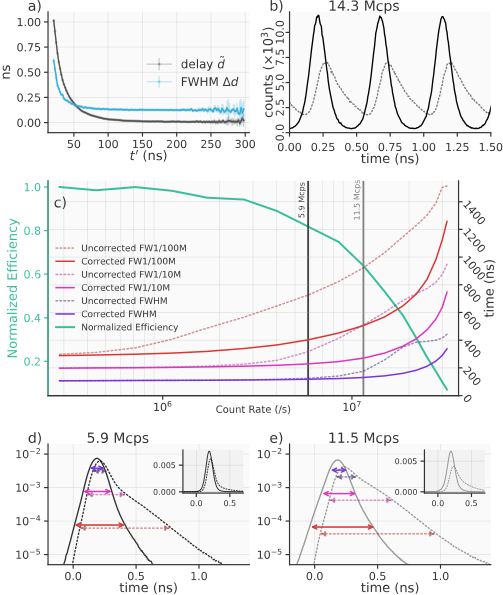
\includegraphics[width=0.7\textwidth,height=\textheight]{chapter_01/./figs/Figure_Data_Sept_2022.svg}
\caption[{The second first caption.}]{\textbf{The caption heading} And I
think the rest of this is the caption}
\label{fig:custom_figure}
\end{figure}
}

\hypertarget{high-rate-pulse-position-modulation}{%
\chapter{High Rate Pulse Position
Modulation}\label{high-rate-pulse-position-modulation}}

~~~~~~~~~~~~~~~~~~~~~~~~~~~~~~\includegraphics{chapter_01/coarse_grain.pdf}

A version of this chapter originally appeared as Razo-Mejia, M.\emph{,
Barnes, S.L.}, Belliveau, N.M.\emph{, Chure, G.}, Einav, T.*, Lewis, M.,
and Phillips, R. (2018). Tuning transcriptional regulation through
signaling: A predictive theory of allosteric induction. Cell Systems 6,
456-469.e10. DOI:https://doi.org/10.1016/j.cels.2018.02.004. M.R.M,
S.L.B, N.M.B, G.C., and T.E. contributed equally to this work from the
theoretical underpinnings to the experimental design and execution.
M.R.M, S.L.B, N.M.B, G.C, T.E., and R.P. wrote the paper. M.L. provided
extensive guidance and advice.

\hypertarget{abstract}{%
\section{Abstract}\label{abstract}}

Allosteric regulation is found across all domains of life, yet we still
lack simple, predictive theories that directly link the experimentally
tunable parameters of a system to its input-output response. To that
end, we present a general theory of allosteric transcriptional
regulation using the Monod-Wyman- Changeux model. We rigorously test
this model using the ubiquitous simple repression motif in bacteria by
first predicting the behavior of strains that span a large range of
repressor copy numbers and DNA binding strengths, and then constructing
and measuring their response. Our model not only accurately captures the
induction profiles of these strains, but also enables us to derive
analytic expressions for key properties such as the dynamic range and
{[}EC\(_{50}\){]}. Finally, we derive an expression for the free energy
of allosteric repressors that enables us to collapse our experimental
data onto a single master curve that captures the diverse phenomenology
of the induction profiles.

\hypertarget{introduction-1}{%
\section{Introduction}\label{introduction-1}}

~~~~~Understanding how organisms sense and respond to changes in their
environment has long been a central theme of biological inquiry. At the
cellular level, this interaction is mediated by a diverse collection of
molecular signaling pathways. A pervasive mechanism of signaling in
these pathways is allosteric regulation, in which the binding of a
ligand induces a conformational change in some target molecule,
triggering a signaling cascade \autocite{lindsley2006a}. One of the most
important examples of such signaling is offered by transcriptional
regulation, where a transcription factors' propensity to bind to DNA
will be altered upon binding to an allosteric effector.

~~~~~Despite the ubiquity of allostery, we largely lack a formal,
rigorous, and generalizable framework for studying its effects across
the broad variety of contexts in which it appears. A key example of this
is transcriptional regulation, in which allosteric transcription factors
can be induced or corepressed by binding to a ligand. An allosteric
transcription factor can adopt multiple conformational states, each of
which has its own affinity for the ligand and for its DNA target site.
\emph{In vitro} studies have rigorously quantified the equilibria of
different conformational states for allosteric transcription factors and
measured the affinities of these states to the ligand
\autocite{harman2001,lanfranco2017}. In spite of these experimental
observations, the lack of a coherent quantitative model for allosteric
transcriptional regulation has made it impossible to predict the
behavior of even a simple genetic circuit across a range of regulatory
parameters, physiological states of the organism, and evolutionary
isoforms of the regulatory sequences.

~~~~~The ability to predict circuit behavior robustly--- that is, across
both broad ranges of parameters and regulatory architectures ---is
important for multiple reasons. First, in the context of a specific
gene, accurate prediction demonstrates that all components relevant to
the genes' behavior have been identified and characterized to sufficient
quantitative precision. Second, in the context of genetic circuits in
general, robust prediction validates the model that generated the
prediction. Possessing a validated model also has implications for
future work. For example, when we have sufficient confidence in the
model, a single data set can be used to accurately extrapolate a
system's behavior in other conditions. Moreover, there is an essential
distinction between a predictive model, which is used to predict a
system's behavior given a set of input variables, and a retroactive
model, which is used to describe the behavior of data that has already
been obtained. We note that even some of the most careful and rigorous
analysis of transcriptional regulation often entails only a retroactive
reflection on a single experiment. This raises the fear that each
regulatory architecture may require a unique analysis that cannot carry
over to other systems, a worry that is exacerbated by the prevalent use
of phenomenological functions (e.g.~Hill functions or ratios of
polynomials) that can analyze a single data set, but cannot be used to
extrapolate a system's behavior in other conditions
\autocite{setty2003,poelwijk2011a,vilar2013,rogers2015,rohlhill2017}.

~~~~~This work explores what happens when theory takes center stage,
namely, we first write down the equations governing a system and
describe its expected behavior across a wide array of experimental
conditions, and only then do we set out to experimentally confirm these
results. Building upon previous work
\autocite{garcia2011,brewster2014,weinert2014} and the work of Monod,
Wyman, and Changeux \autocite{monod1965}, we present a statistical
mechanical rendering of allostery in the context of induction and
corepression (shown schematically in Fig.~\ref{fig:inducible_types} and
henceforth referred to as the MWC model), and use it as the basis of
parameter-free predictions which we then test experimentally. More
specifically, we study the simple repression motif -- a widespread
bacterial genetic regulatory architecture in which binding of a
transcription factor occludes binding of an RNA polymerase, thereby
inhibiting transcription initiation. The MWC model stipulates that an
allosteric protein fluctuates between two distinct conformations -- an
active and inactive state -- in thermodynamic equilibrium
\autocite{monod1965}. During induction, for example, effector binding
increases the probability that a repressor will be in the inactive
state, weakening its ability to bind to the promoter and resulting in
increased expression. To test the predictions of our model across a wide
range of operator binding strengths and repressor copy numbers, we
design a genetic construct in \emph{Escherichia coli} in which the
binding probability of a repressor regulates gene expression of a
fluorescent reporter.

~~~~~In total, the work presented here demonstrates that one extremely
compact set of parameters can be applied self-consistently and
predictively to different regulatory situations including simple
repression on the chromosome, cases in which decoy binding sites for
repressor are put on plasmids, cases in which multiple genes compete for
the same regulatory machinery, cases involving multiple binding sites
for repressor leading to DNA looping, and induction by signaling
\autocite{garcia2011,garcia2011b,brewster2012,brewster2014,boedicker2013a,boedicker2013}.
Thus, rather than viewing the behavior of each circuit as giving rise to
its own unique input-output response, the MWC model provides a means to
characterize these seemingly diverse behaviors using a single unified
framework governed by a small set of parameters.

\hypertarget{fig:inducible_types}{%
\begin{figure}
\centering
\includegraphics{chapter_01/ch2_fig1.pdf}
\caption[{Transcriptional regulatory architectures involving an
allosteric repressor.}]{\textbf{Transcriptional regulatory motifs
involving an allosteric repressor.} (A) We consider a promoter regulated
solely by an allosteric repressor in which the active (repressive, red
blobs) state of the repressor is energetically favorable in the absence
(induction, left panel) or presence (corepression, right panel) of an
allosteric effector. Both inducible repression and corepression are
ubiquitous regulatory strategies in \emph{E. coli}, several examples of
which are given in the tables below each panel. (B) A representative
regulatory response (fold-change in gene expression) of the two
architectures shown in Panel (A) as a function of the corresponding
allosteric effector concentration. Properties of interest to this work
are shown schematically upon the regulatory response. (C) Historical
progression of thermodynamic modeling of the inducible simple-repression
regulatory architecture. \textcite{garcia2011} used colorimetric assays
and quantitative Western blots to investigate how single-site repression
is modified by the repressor copy number and repressor-DNA binding
energy. \textcite{brewster2014} used video microscopy to probe how the
copy number of the promoter and presence of competing repressor binding
sites affect gene expression. Building upon these works, we use flow
cytometry to determine the inducer-repressor dissociation constants and
demonstrate that with these parameters we can predict \emph{a priori}
the behavior of the system for any repressor copy number, DNA binding
energy, gene copy number, and inducer concentration.}
\label{fig:inducible_types}
\end{figure}
}

\hypertarget{time-walk-and-jitter-correction}{%
\chapter{Time Walk and Jitter
Correction}\label{time-walk-and-jitter-correction}}

~~~~~~~~~\includegraphics{chapter_01/mutant.pdf}

A version of this chapter originally appeared as Chure, G, Razo-Mejia,
M., Belliveau, N.M., Kaczmarek, Zofii A., Einav, T., Barnes, Stephanie
L., Lewis, M., and Phillips, R. (2019). Predictive shifts in free energy
couple mutations to their phenotypic consequences. Proceedings of the
National Academies of Sciences 116(37) DOI:
https://doi.org/10.1073/pnas.1907869116. G.C., M.R.M, N.M.B., Z.A.K.,
and S.L.B designed the experiments and collected and analyzed data. G.C.
developed the theoretical treatment of free energy shifts. G.C., M.R.M,
N.M.B., Z.A.K., T.E., S.L.B., and R.P. designed the research project.
G.C. and R.P. wrote the paper. M.L. provided guidance and advice.

\hypertarget{abstract-1}{%
\section{Abstract}\label{abstract-1}}

Mutation is a critical mechanism by which evolution explores the
functional landscape of proteins. Despite our ability to experimentally
inflict mutations at will, it remains difficult to link sequence-level
perturbations to systems-level responses. Here, we present a framework
centered on measuring changes in the free energy of the system to link
individual mutations in an allosteric transcriptional repressor to the
parameters which govern its response. We find that the energetic effects
of the mutations can be categorized into several classes which have
characteristic curves as a function of the inducer concentration. We
experimentally test these diagnostic predictions using the
well-characterized LacI repressor of \emph{Escherichia coli}, probing
several mutations in the DNA binding and inducer binding domains. We
find that the change in gene expression due to a point mutation can be
captured by modifying only the model parameters that describe the
respective domain of the wild-type protein. These parameters appear to
be insulated, with mutations in the DNA binding domain altering only the
DNA affinity and those in the inducer binding domain altering only the
allosteric parameters. Changing these subsets of parameters tunes the
free energy of the system in a way that is concordant with theoretical
expectations. Finally, we show that the induction profiles and resulting
free energies associated with pairwise double mutants can be predicted
with quantitative accuracy given knowledge of the single mutants,
providing an avenue for identifying and quantifying epistatic
interactions.

\hypertarget{introduction-2}{%
\section{Introduction}\label{introduction-2}}

~~~~~ To be written

\hypertarget{the-peacoq-detector-and-higher-order-correction-methods}{%
\section{The Peacoq Detector, and Higher Order Correction
Methods}\label{the-peacoq-detector-and-higher-order-correction-methods}}

\hypertarget{outlook-towards-high-rate-pnr-and-time-walk-correction}{%
\section{Outlook: Towards High Rate PNR and Time Walk
Correction}\label{outlook-towards-high-rate-pnr-and-time-walk-correction}}

\hypertarget{high-rate-entanglement-generation}{%
\chapter{High Rate Entanglement
Generation}\label{high-rate-entanglement-generation}}

~~~~~~~~~~~~~~~~~~~~~~~~~~~~~~~~~~~~\includegraphics{chapter_01/physiology.pdf}

A version of this chapter is currently under review. A preprint is
released as Chure, G, Kaczmarek, Z. A., and Phillips, R. Physiological
adaptability and parametric versatility in a simple genetic circuit.
bioRxiv 2019. DOI: 10.1101/2019.12.19.878462. G.C. and R.P. designed
experiments and developed theoretical models. G.C. and Z.A.K. collected
and analyzed data. G.C. and R.P. wrote the paper.

\hypertarget{abstract-2}{%
\section{Abstract}\label{abstract-2}}

The intimate relationship between the environment and cellular growth
rate has remained a major topic of inquiry in bacterial physiology for
over a century. Now, as it becomes possible to understand how the growth
rate dictates the wholesale reorganization of the intracellular
molecular composition, we can interrogate the biophysical principles
underlying this adaptive response. Regulation of gene expression drives
this adaptation, with changes in growth rate tied to the activation or
repression of genes covering enormous swaths of the genome. Here, we
dissect how physiological perturbations alter the expression of a
circuit which has been extensively characterized in a single
physiological state. Given a complete thermodynamic model, we map
changes in physiology directly to the biophysical parameters which
define the expression. Controlling the growth rate via modulating the
available carbon source or growth temperature, we measure the level of
gene expression from a LacI-regulated promoter where the LacI copy
number is directly measured in each condition, permitting parameter-free
prediction of the expression level. The transcriptional output of this
circuit is remarkably robust, with expression of the repressor being
largely insensitive to the growth rate. The predicted gene expression
quantitatively captures the observations under different carbon
conditions, indicating that the biophysical parameters are indifferent
to the physiology. Interestingly, temperature controls the expression
level in ways that are inconsistent with the prediction, revealing
temperature-dependent effects that challenge current models. This work
exposes the strengths and weaknesses of thermodynamic models in
fluctuating environments, posing novel challenges and utility in
studying physiological adaptation.

\hypertarget{introduction-3}{%
\section{Introduction}\label{introduction-3}}

Cellular physiology is inextricably tied to the extracellular
environment. Fluctuations in nutrient availability and variations in
temperature, for example, can drastically modulate the cell's growth
rate, which is often used as a measure of the evolutionary fitness
\autocite{schaechter1958}. In response to such environmental insults,
cells have evolved myriad clever mechanisms by which they can adapt to
their changing surroundings, many of which involve restructuring their
proteome such that critical processes (i.e.~protein translation) are
allocated the necessary resources. Recent work exploring this level of
adaptation using mass spectrometry, ribosomal profiling, and RNA
sequencing have revealed that various classes of genes (termed
``sectors'') are tuned such that the protein mass fraction of the
translational machinery is prioritized over the metabolic and catabolic
machinery in nutrient replete environments
\autocite{scott2014,klumpp2014,hui2015,schmidt2016,li2014}. This drastic
reorganization is mediated by the regulation of gene expression, relying
on the concerted action of myriad transcription factors. Notably, each
gene in isolation is regulated by only one or a few components
\autocite{gama-castro2016}. The most common regulatory architecture in
\emph{Escherichia coli} is the simple repression motif in which a
transcriptional repressor binds to a single site in the promoter region,
occluding binding of an RNA polymerase
\autocite{rydenfelt2014,phillips2019}. The simple activation
architecture, in which the simultaneous binding of an activator and an
RNA polymerase amplifies gene expression, is another common mode of
regulation. Combinatorial regulation such as dual repression, dual
activation, or combined activation and repression can also be found
throughout the genome, albeit with lower frequency
\autocite{phillips2019}. The ubiquity of the simple repression and
simple activation motifs illustrate that, for many genes, the complex
systems-level response to a physiological perturbation boils down the
binding and unbinding of a single regulator to its cognate binding
sites.

~~~~~Despite our knowledge of these modes of regulation, there remains a
large disconnect between concrete, physical models of their behavior and
experimental validation. The simple repression motif is perhaps the most
thoroughly explored theoretically and experimentally
\autocite{phillips2019} where equilibrium thermodynamic
\autocite{garcia2011,garcia2012,brewster2014,razo-mejia2018,barnes2019}
and kinetic \autocite{jones2014,ko1991,kepler2001,michel2010} models
have been shown to accurately predict the level of gene expression in a
variety of contexts. While these experiments involved variations of
repressor copy number, operator sequence, concentration of an external
inducer, and amino acid substitutions, none have explored how the
physiological state of the cell as governed by external factors
influences gene expression. This is arguably one of the most critical
variables one can experimentally tune to understand the roles these
regulatory architectures play in cellular physiology writ large.

~~~~~In this work, we interrogate the adaptability of a simple genetic
circuit to various physiological stressors, namely carbon source quality
and growth temperature. Following the aforementioned thermodynamic
models, we build upon this theory-experiment dialogue by using
environmental conditions as an experimentally tunable variable and
determine their influence on various biophysical parameters.
Specifically, we use physiological stressors to tune the growth rate.
One mechanism by which we modulate the growth rate is by exchanging
glucose in the growth medium for the poorer carbon sources glycerol and
acetate, which decrease the growth rate by a factor of \(\approx\) 1.5
and \(\approx\) 4 compared to glucose, respectively. We hypothesize that
different carbon sources should, if anything, only modulate the
repressor copy number seeing as the relationship between growth rate and
total protein content has been rigorously quantified
\autocite{schaechter1958,schmidt2016,li2014,jun2018}. Using single-cell
time-lapse fluorescence microscopy, we directly measure the copy number
of the repressor in each condition. Under a simple hypothesis, all other
parameters should be unperturbed, and we can thus rely on previously
determined values to make parameter-free predictions of the fold-change
in gene expression.

~~~~~Despite the decrease in growth rate, both the fold-change in gene
expression and the repressor copy number remains largely unaffected. We
confirm this is the case by examining how the effective free energy of
the system changes between carbon sources, a method we have used
previously to elucidate parametric changes due to mutations within a
transcription factor \autocite{chure2019} and has been extensively
discussed in Chapter 3. This illustrates that the energetic parameters
defining the fraction of active repressors and their affinity for the
DNA are ignorant of the carbon-dependent physiological states of the
cell. Thus, in this context, the values of the biophysical parameters
determined in one condition can be used to draw predictions in others.

~~~~~We then examine how variations in temperature influence the
transcriptional output. Unlike in the case of carbon source variation,
temperature dependence is explicit in our model: the repressor-DNA
binding energy and the energetic difference between the active and
inactive states of the repressor are scaled to the thermal energy of the
system at 37\(^\circ\) C. This is defined via the Boltzmann distribution
which states that the probability of a state \(p_{state}\) is related to
the energy of that state \(\varepsilon_{state}\) as
\begin{equation}\protect\hypertarget{eq:boltz}{}{
p_{state} \propto e^{-\varepsilon_{state} / k_BT},
}\label{eq:boltz}\end{equation} where \(k_B\) is the Boltzmann constant
and \(T\) is the temperature of the system. Given knowledge of \(T\) for
a particular experiment, we can easily draw predictions of the
fold-change in gene expression. However, we find that the fold-change in
gene expression is inconsistent with this simple model, revealing an
incomplete description of the energetics. We then examine how entropic
effects neglected in the initial estimation of the energetic parameters
may play an important role; a hypothesis that is supported when we
examine the change in the effective free energy.

~~~~~

\hypertarget{appendix-1}{%
\chapter{Appendix 1}\label{appendix-1}}

~~~~~~~~~~~~~\includegraphics{chapter_01/coming_storm.pdf}

A version of this chapter was published as Chure, G.* , Lee, H.J.\emph{,
Rasmussen, A., and Phillips, R. (2018). Connecting the dots between
mechanosensitive channel abundance, osmotic shock, and survival at
single-cell Resolution. Journal of Bacteriology 200. DOI:
10.1128/JB.00460-18 (} contributed equally). G.C., H.J.L, and R.P.
designed and planned experiments. G.C. and H.J.L performed experiments.
H.J.L constructed bacterial strains. A.R. performed electrophysiology
experiments. G.C. performed data analysis and figure generation. G.C.
and R.P. wrote the manuscript.

\hypertarget{abstract-3}{%
\section{Abstract}\label{abstract-3}}

Rapid changes in extracellular osmolarity are one of many insults
microbial cells face on a daily basis. To protect against such shocks,
\emph{Escherichia coli} and other microbes express several types of
transmembrane channels that open and close in response to changes in
membrane tension. In \emph{E. coli}, one of the most abundant channels
is the mechanosensitive channel of large conductance (MscL). While this
channel has been heavily characterized through structural methods,
electrophysiology, and theoretical modeling, our understanding of its
role in preventing cell death due to osmotic shock remains tenuous. In
this work, we examine the contribution of MscL alone to cell survival
after osmotic shock at single-cell resolution using quantitative
fluorescence microscopy. We conducted these experiments in an \emph{E.
coli} strain which is lacking all mechanosensitive channel genes save
for MscL, whose expression was tuned across 3 orders of magnitude
through modifications of the Shine-Dalgarno sequence. While theoretical
models suggest that only a few MscL channels would be needed to
alleviate even large changes in osmotic pressure, we find that between
500 and 700 channels per cell are needed to convey upwards of 80\%
survival. This number agrees with the average MscL copy number measured
in wild-type \emph{E. coli} cells through proteomic studies and
quantitative Western blotting. Furthermore, we observed zero survival
events in cells with fewer than \(\approx\) 100 channels per cell. This
work opens new questions concerning the contribution of other
mechanosensitive channels to survival, as well as regulation of their
activity.

\hypertarget{introduction-4}{%
\section{Introduction}\label{introduction-4}}

Changes in the extracellular osmolarity can be a fatal event for the
bacterial cell. Upon a hypo-osmotic shock, water rushes into the cell
across the membrane, leaving the cell with no choice but to equalize the
pressure. This equalization occurs either through damage to the cell
membrane (resulting in death) or through the regulated flux of water
molecules through transmembrane protein channels (Fig 1A). Such
proteinaceous pressure release valves have been found across all domains
of life, with the first bacterial channel being described in 1987
\autocite{martinac1987}. Over the past thirty years, several more
channels have been discovered, described, and (in many cases)
biophysically characterized. \emph{E. coli}, for example, has seven of
these channels (one MscL and six MscS homologs) which have varied
conductance, gating mechanisms, and expression levels. While they have
been the subject of much experimental and theoretical dissection, much
remains a mystery with regard to the roles their abundance and
interaction with other cellular processes play in the greater context of
physiology
\autocite{bavi2016,bialecka-fornal2012,bialecka-fornal2015,edwards2012,naismith2012,ursell2008,vandenberg2016}.

~~ ~ ~Of the seven channels in \emph{E. coli}, the mechanosensitive
channel of large conductance (MscL) is one of the most abundant and the
best characterized. This channel has a large conductance (3 nS) and
mediates the flux of water molecules across the membrane via a
\textasciitilde3 nm wide pore in the open state
\autocite{cruickshank1997,haswell2011}. Molecular dynamics simulations
indicate that a single open MscL channel permits the flux of
\(4 \times 10^9\) water molecules per second, which is an order of
magnitude larger than a single aquaporin channel (BNID 100479)
\autocite{louhivuori2010,milo2010}. This suggests that having only a few
channels per cell could be sufficient to relieve even large changes in
membrane tension. Electrophysiological experiments have suggested a
small number of channels per cell \autocite{booth2005,hase1997},
however, more recent approaches using quantitative Western blotting,
fluorescence microscopy, and proteomics have measured several hundred
MscL per cell \autocite{bialecka-fornal2012,schmidt2016,soufi2015}. To
further complicate matters, the expression profile of MscL appears to
depend on growth phase, available carbon source, and other environmental
challenges
\autocites[\textcite{schmidt2016}]{bialecka-fornal2012}{soufi2015,stokes2003}.
While there are likely more than just a few channels per cell, why cells
seem to need so many and the biological rationale behind their
condition-dependent expression both remain a mystery.

~~~ ~ While their biochemical and biophysical characteristics have
received much attention, their connection to cell survival is
understudied. Drawing such a direct connection between channel copy
number and survival requires quantitative \emph{in vivo} experiments. To
our knowledge, the work presented in \autocite{vandenberg2016} is the
first attempt to simultaneously measure channel abundance and
survivability for a single species of mechanosensitive channel. While
the measurement of channel copy number was performed at the level of
single cells using super-resolution microscopy, survivability after a
hypo-osmotic shock was assessed in bulk plating assays which rely on
serial dilutions of a shocked culture followed by counting the number of
resulting colonies after incubation. Such bulk assays have long been the
standard for querying cell viability after an osmotic challenge. While
they have been highly informative, they reflect only the mean survival
rate of the population, obfuscating the variability in survival of the
population. The stochastic nature of gene expression results in a noisy
distribution of MscL channels rather than a single value, meaning those
found in the long tails of the distribution have quite different
survival rates than the mean, but are lost in the final calculation of
survival probability.

~ ~ ~ ~In this work, we present an experimental system to quantitatively
probe the interplay between MscL copy number and survival at single-cell
resolution, as is seen in Fig.~\ref{fig:overview}(B). We generated an
\emph{E. coli} strain in which all seven mechanosensitive channels had
been deleted from the chromosome followed by a chromosomal integration
of a single gene encoding an MscL-super-folder GFP (sfGFP) fusion
protein. To explore copy number regimes beyond those of the wild-type
expression level, we modified the Shine-Dalgarno sequence of this
integrated construct, allowing us to cover nearly three decades of MscL
copy number. To probe survivability, we exposed cells to a large
hypo-osmotic shock at controlled rates in a flow cell under a
microscope, allowing the observation of the single-cell channel copy
number and the resulting survivability of single cells. With this large
set of single cell measurements, we approach the calculation of survival
probability in a manner that is free of binning bias which allows the
reasonable extrapolation of survival probability to copy numbers outside
of the observed range. In addition, we show that several hundred
channels are needed to convey high rates of survival and observe a
minimum number of channels needed to permit any degree of survival.

\hypertarget{fig:overview}{%
\begin{figure}
\centering
\includegraphics{chapter_01/ch5_fig1.pdf}
\caption[{Role of mechanosensitive channels during hypo-osmotic
shock.}]{\textbf{Role of mechanosensitive channels during hypo-osmotic
shock.} (A) A hypo-osmotic shock results in a large difference in the
osmotic strength between the intracellular and extracellular spaces. As
a result, water rushes into the cell to equalize this gradient
increasing the turgor pressure and tension in the cell membrane. If no
mechanosensitive channels are present and membrane tension is high (left
panel), the membrane ruptures releasing intracellular content into the
environment resulting in cell death. If mechanosensitive channels are
present (right panel) and membrane tension is beyond the gating tension,
the mechanosensitive channel MscL opens, releasing water and small
intracellular molecules into the environment, thus relieving pressure
and membrane tension. (B) The experimental approach undertaken in this
work. The number of mechanosensitive channels tagged with a fluorescent
reporter is tuned through modification of the Shine-Dalgarno sequence of
the \emph{mscL} gene. The cells are then subjected to a hypo-osmotic
shock and the number of surviving cells are counted, allowing the
calculation of a survival probability.}
\label{fig:overview}
\end{figure}
}

\hypertarget{software-systems-and-operation}{%
\section{Software Systems and
Operation}\label{software-systems-and-operation}}

\printbibliography
\end{document}
